\section {Interaction Design}
During the ROLE-project many sketches have been developed by different contributors. These contributors include, but is not limited to, Uppsala Learning Lab. This section will start by analysing the sketches presented in the previous work section (section 2.5.1). The information gathered from the analysis will be used together with the results from the personas to create new design sketches.

In the ROLE-project most designs are quite similar. This thesis focuses on the designs made by Uppsala Learning Lab as they requested the evaluations.

\subsection {Analysis  of Previous Designs}
The analyses in this section are my personal reflections made with the aid of the ten rules of heuristics listed in the previous work section (section 2.5).

Looking at the sketches made earlier by Uppsala Learning Lab it is clear that a certain concept is being followed. Each course is supposed to have a separate workspace to which widgets can be attached. These tools does not appear in other spaces, and these widgets can not communicate with other widgets outside of the current workspace. This could become a problem if information is to be transferred from one course to another. The solution is a personal widget area which is available on each workspace. This area follows the user to all of his or her workspaces.

In the first version one could argue that the personal area takes too much space. Not allowing the widgets in the workspace enough room. In the second version this is clearly visible. The only reason the image looks somewhat usable is because it is not formatted to a computer screen. When viewing the design on a regular (4:3) monitor the workspace is either be empty on the right or left side or the user would have to scroll down to access the personal area. This effect is even more apparent when viewing on a wide-screen (16:9) monitor. This issue has been addressed in the third version. Here the personal area has been modified into a personal toolbar instead, allowing either more widgets or bigger widgets.

In the first and second version there are indicators next to the widget names on the navigation bars. These are supposed to show the user when widget communications are initiated and received. In the first version these are marked by coloured icons. There are two problems with these icons: The first problem is that the icons take no consideration of the colour blind who may not be able to distinguish between two actions. The other problems is that it is not certain whether these icons are needed in the first place.  This creates a conflict with the first and fifth rule of heuristics. One saying that no extra information should be shown as it may cause confusion and the other saying that the user should always be given feedback on what is going on inside the program. The first problem has been addressed in the second version where arrows have replaced the icons to indicate the direction of the communications. The icons and arrows have been removed in the third design removing the possibility of icons confusing students. Feedback is given by marking new events inside a widget with a new colour and contrast. It is unclear from the sketch if this would be visible if the widget is minimized.

Looking at the first version widgets are opened and minimized using check boxes. This may not be an obvious way to everyone at a first glance but users should not need more than one demonstration to remember it. One issue is that check boxes are not always that easy to click. It should therefore be possible to check and uncheck the box and open widgets by clicking the widget name as well as the check box. In the second and third version these check boxes are not present. According to the people at Uppsala Learning Lab this is not intentional, it has simply not been added yet. The same goes for the ability to add widgets which in the first sketch is done by clicking “edit” in the navigation area. It is very important that this feature is done correctly and in an obvious way since the whole concept of the widget based system is that students are able to find and add widgets that suit them best.

Summarizing the three versions there are some ideas to reuse and some to add.
\begin {itemize}
	\item Divide the working space into a course-specific area and one personal area.
	\item The personal area should not take too much space. A toolbar is one way of doing this.
	\item Adding and removing widgets should be easy to do.
	\item How to open and minimize/close widgets should be obvious.
	\item Widget communications should be visible, but should not interfere with the user's focus.
\end {itemize}

\subsection {New Design Sketches}
These sketches are derived from the sketches made by Uppsala Learning Lab with the ideas from the end of the last section implemented. The sketches are made with the free version of the commercial tool balsamiq. 
The main idea is to have the widget area as large as possible. The widgets should then place themselves inside the widget area when opened. Widgets are never closed, they are just minimized and the information should be available the next time the widget is opened. The widgets are managed by a navigation bar on the side where other resources as fellow students and teachers can be found. At the bottom there is a bar containing the personal widgets.

There are two types of spaces, one is a course space. This space is created by the teacher with a copy distributed to all students. The students will receive the copy at the start of the course. This space will contain widgets recommended by the teacher. The students now have the option to add his or her own favourite widgets in order to make the widget area personally optimized. The other type of space is an empty space where students can create their own space from an empty template. If a student finds his or her space very useful it is possible to share copies of the space to fellow students and also invite fellow students to the space for group assignments and other group activities.

\pagebreak
\begin{figure}[h]
	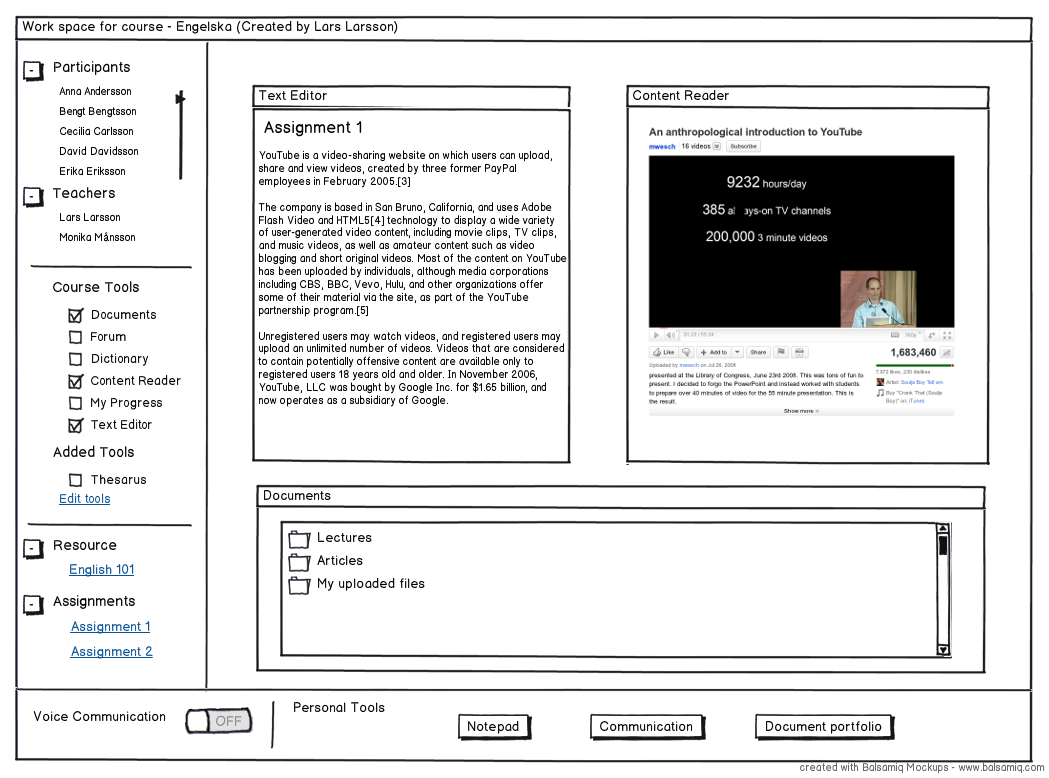
\includegraphics[width=1.0\textwidth] {mj_course.png}
	\caption {Concept sketch of a widget space for a course}
	\label {fig:mj_course.png}
\end{figure}

In the course version the teachers have selected some recommended widgets as a basic version. The student then has the option to add a widget by clicking the link “Edit tools”. The tools added in this design are quite self-explanatory which could be useful when separating a large system into widgets. There is however one widget that may not be so intuitive just by looking at the name. The content reader is a widget that displays contextual information. If a link is clicked in another widget the content reader will fetch the information from that link. If, for example, a YouTube link is visited the content reader will extract the video from the site and only show that instead of displaying the whole page.

\pagebreak
\begin{figure}[h]
	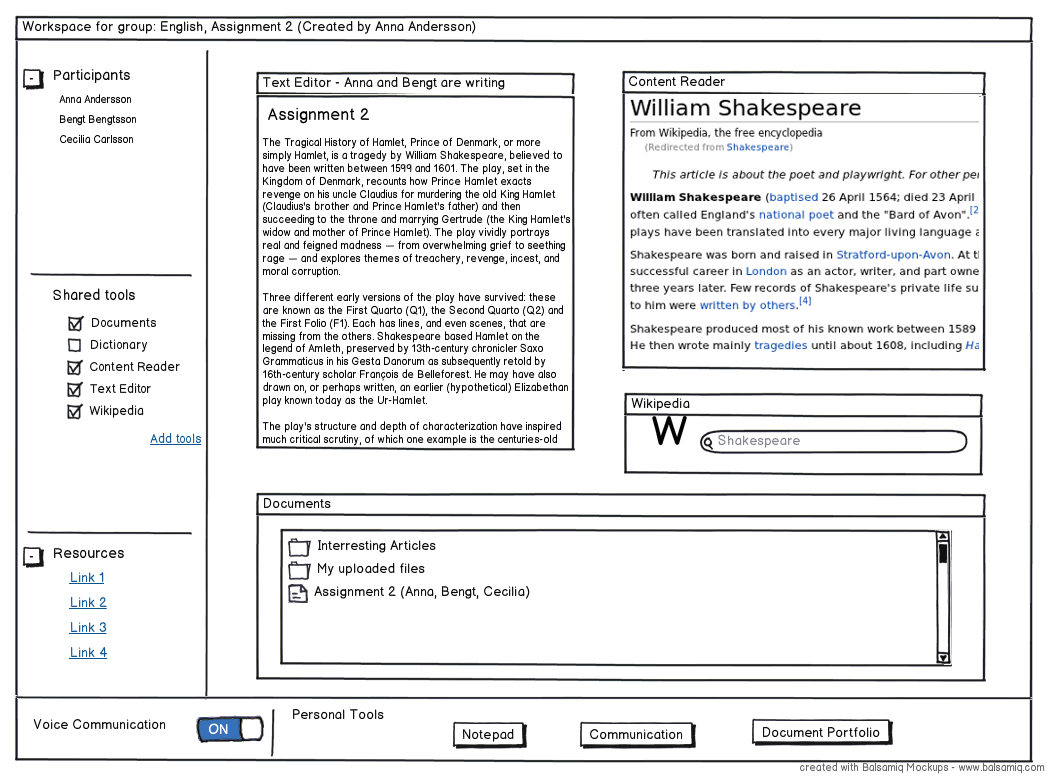
\includegraphics[width=1.0\textwidth] {mj_group.png}
	\caption {Concept sketch of a widget space for a group}
	\label {fig:mj_course.png}
\end{figure}

The empty space version is here implemented as a group version. A student has created a new work space and shared it with two fellow students for an assignment. Together they add widgets they find useful and write their assignment in the collaborative text editor. The functionality of the content reader is visible here. After a search in the Wikipedia-widget the content browser will fetch the requested article from Wikipedia and display it. 

The personal toolbar is the same in both versions to show that it is independent from the current work space and is the same everywhere in the system. The personal toolbar will have to be edited in a special screen. This could be done from a personal menu screen where other personal settings are edited and where workspaces are managed.
